\subsection{Module 4: Yêu cầu tạo tin mới, quản lý các tin đã gửi}
\subsubsection{Thêm mới}
\begin{figure}[H]
	\centering
	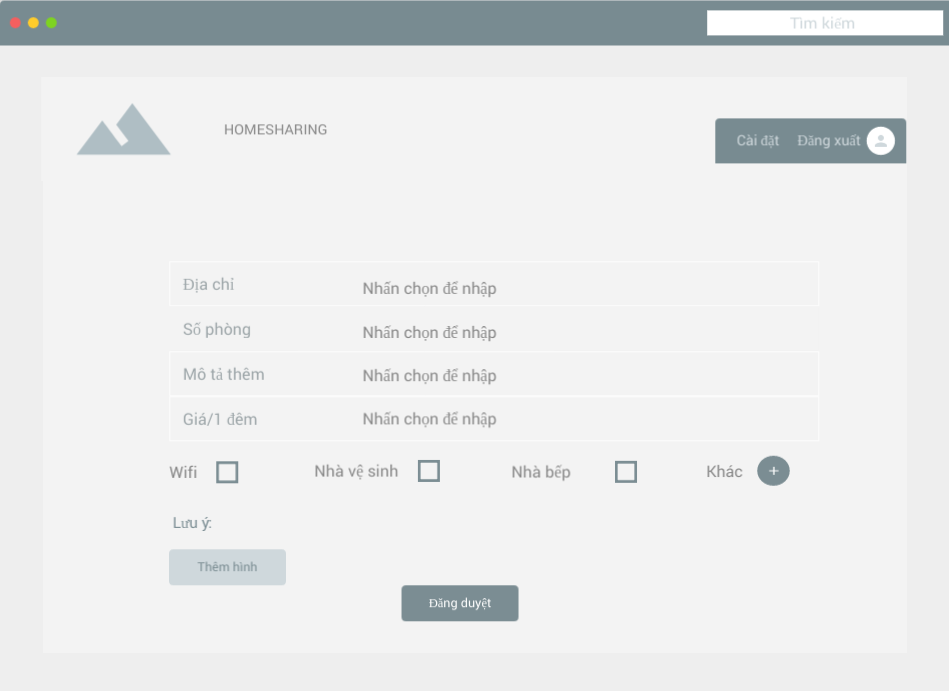
\includegraphics[width=10cm]{parts/bao/images/createPost.png}
	\vspace{0.5cm}
	\caption{UI tạo mới một tin}
\end{figure}

\subsubsection{Xem danh sách tin}
\begin{figure}[H]
	\centering
	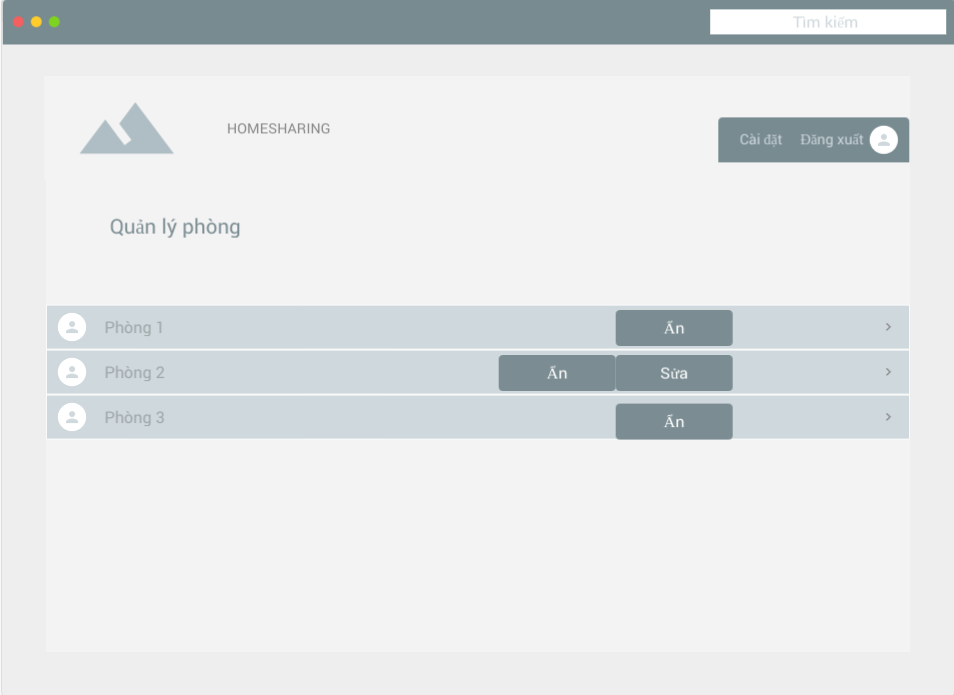
\includegraphics[width=10cm]{parts/bao/images/roomManager.png}
	\vspace{0.5cm} 
	\caption{UI xem danh sách tin}
\end{figure}
\newpage 
\subsubsection{Chỉnh sửa tin đã đăng}
\begin{figure}[H]
	\centering
	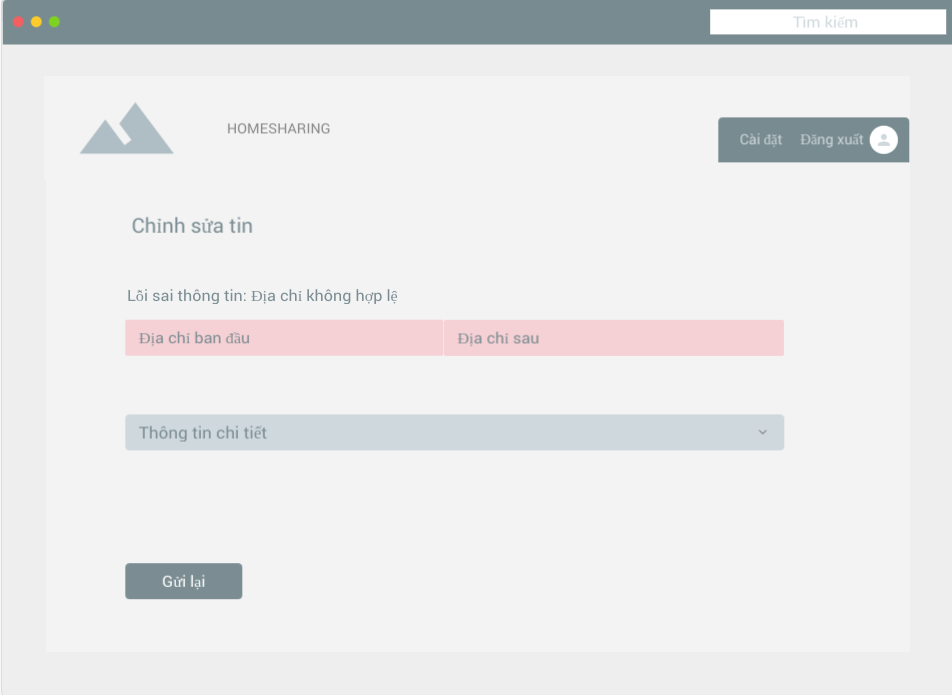
\includegraphics[width=10cm]{parts/bao/images/resendPost.png}
	\vspace{0.5cm} 
	\caption{UI chỉnh sửa tin đã đăng}
\end{figure}

\subsubsection{Ẩn tin đã đăng}
\begin{figure}[H]
	\centering
	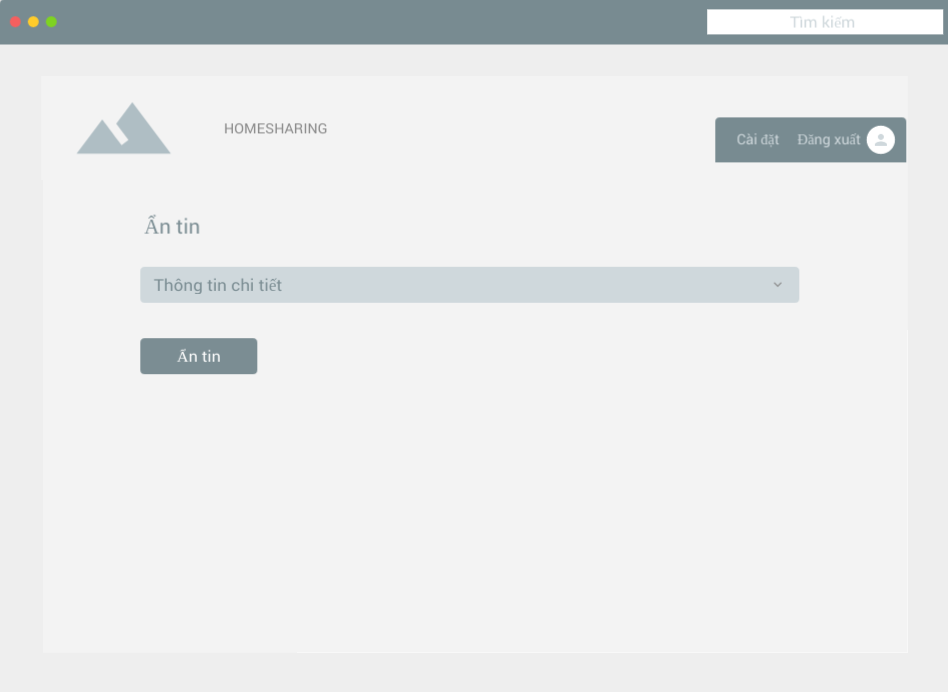
\includegraphics[width=10cm]{parts/bao/images/hidePost.png}
	\vspace{0.5cm} 
	\caption{UI Ẩn một in đã đăng}
\end{figure}%